%%-----------------Chapter 4---------------------------
% \documentclass[../UNBThesis2.tex]{subfiles}
% \usepackage{adjustbox/}
% \usepackage{array,booktabs}
\setlength{\parindent}{2em}
% \begin{document}

\chapter{Data Stream Affinity Propagation}
%This chapter introduces a conceptual framework capable to process data stream clustering using a sliding time window model. 

%This Chapter introduces the Data Stream Affinity Propagation (DSAP) algorithm as a novel data stream clustering algorithm that uses the sliding time window model for data analysis. 

%While most of the current data stream algorithms can process a specific form of data, our proposed DSAP is capable of handling any form of streaming data. In addition, its ability to extract summary information from a large number of internet of things (IoT) sensors made the model more powerful compare to other algorithms. 

This Chapter describes the research methodology adopted for developing, implementing, and evaluating the proposed Data Stream Affinity Propagation (DSAP) algorithm using the landmark time window model. This algorithm is based on previous research work where the online-offline clustering phases have been suggested to overcome the clustering limitations such as detecting abrupt and gradual changes as soon as they occur, and distinguishing drift from noise. Figure \ref{wrk1} provides an overview of the methodology which can be described as follows:

%We introduce the algorithm of DSAP and compare it with the established streaming K-means algorithm. The sliding time window model is used in a clustering data stream in this work to handle the recent data. The three main phases that a stream clustering algorithm employs are as follow. They are depicted in 

\begin{itemize}
    \item\textbf{DSAP Clustering Phase:} computes micro-clusters using a landmark time window model to harvest data streams.  It also computes macro-clusters by re-clustering all the centroids of the micro-clusters found in each time window. The goal is to discover hidden dense clusters structures from indoor localization data streams.
    
    \item\textbf{Intrinsic Clustering Validation Phase}: assesses the quality of the clustering results when there is no ground true label of data. The selected metrics are silhouette index, Caliński-Harabasz index, and Davies-Bouldin index. The focus is to assess between-clusters dispersion and inter-cluster dispersion for all clusters. 
    
    
    
 \begin{figure}[h!]
\centering
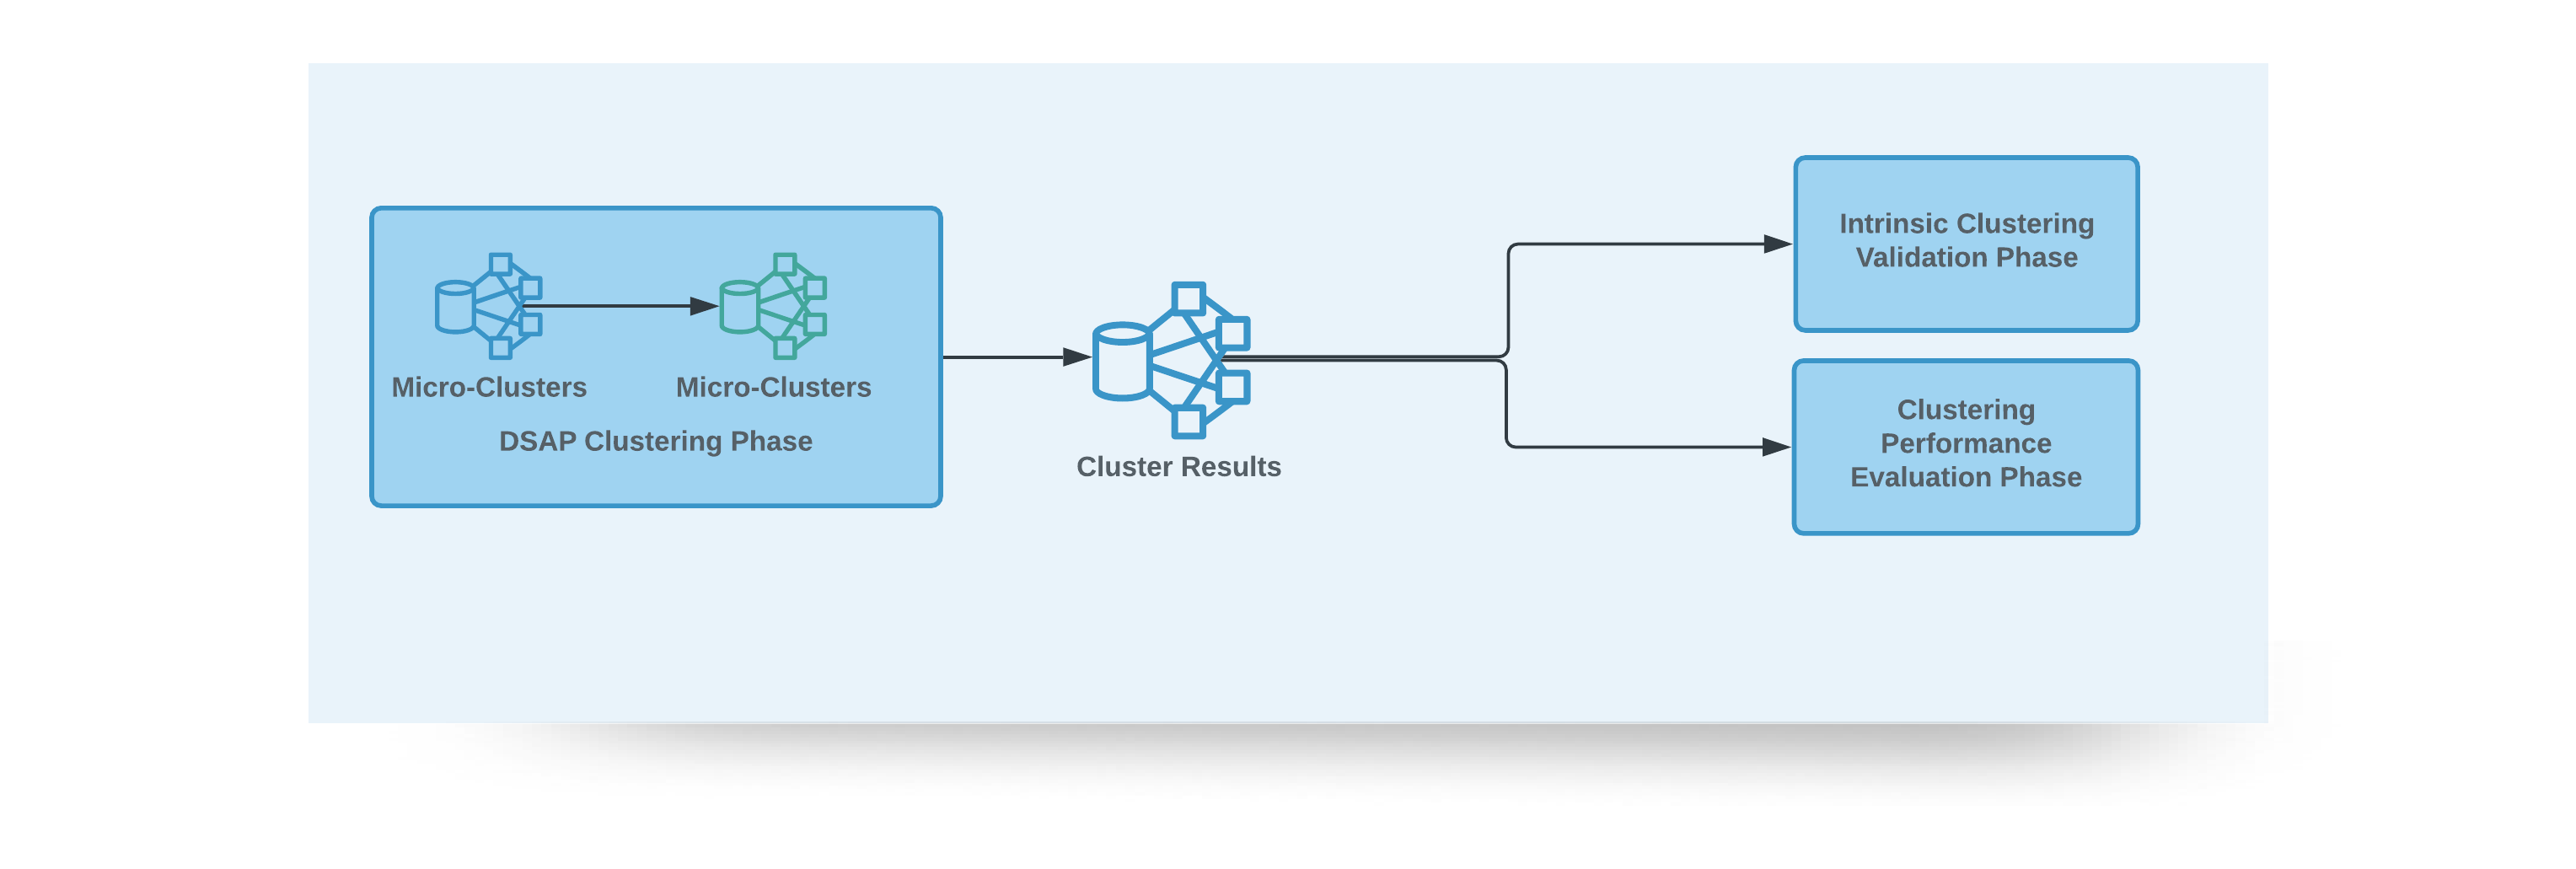
\includegraphics[width = 16 cm]{image/Chapters/Chapter4/phaseDiagram.png} %Blank diagram6
\caption{Overview of the DSAP Phases}
\label{wrk1}
\end{figure}
   
    \item\textbf{Clustering Performance Evaluation Phase:} estimates the efficiency of the DSAP algorithm using the time and space complexity metrics. The aim is to find the right balance between memory consumption and the speed of execution for the DSAP algorithm.
    
   % \item\textbf{Comparison between DSAP and streaming K-means Phase}: The aim is to demonstrate the relevance of the proposed DSAP approach compared to streaming K-means algorithm.
    
\end{itemize}




These phases are described in more detail in the following sections. First, The DSAP clustering phase, with two phases, online micro-cluster and offline macro-cluster, is introduced. Then, the clustering validation and performance evaluation phases are explained.



%%%%%%%%%%%%%%%%%%%%%%%%%%%%%%%%%%%%


%Data stream micro-clustering phase requires a process for saving the summary statistics of a data stream in a fast manner. The online part has a responsibility to maintain the micro clusters of the stream objects. The offline phase uses the last stage summary statistics to provide the user with a fast understanding of the clusters whenever the user submits the request \cite{xu2017fat}.The offline component uses online micro-clustering to find macro clusters.In the next section, first, the sliding time window used in this work will introduce, and then the DSAP data stream clustering will be proposed. In the following, the streaming K-means will be discussed. 



\section{The DSAP Clustering Phase}
The DSAP algorithm is based on the online and offline clustering phases. The online micro-cluster phase detects newly arriving data points and updates the historical clusters accordingly. The offline macro-cluster phase generates summary clusters from the centroids of the micro-clusters at the end of the data stream. 




\subsection{Online Micro-Cluster Phase}

%The online clustering phase initializes a set of micro-clusters with centroids and subsequently analyzes the latest data stream by applying the landmark time window model in a continuous manner that gives updated micro-clusters. (THIS PARAGRAPH DOES NOT MAKE SENSE)
 The online micro-cluster phase initializes by receiving data streams as a continuous sequence of data points that are harvested using the landmark time window model. Therefore, the specifications for creating a landmark time window are its start time and landmark duration $L$ with $\Omega$ data points, where
 $x_i$ is the $i^{th}$ data point in the $j^{th}$ window ($W_j$) in such a way that
 
  \begin{equation}
W_j = \begin{cases}
    0 \quad \phantom{\infty}\text{: if}\,\, i < \Omega  \\
    x_{i+(j-1)*\Omega} \quad \phantom{}  \text{, where $i$=1,2,...,$\Omega$}\,\, :Otherwise  \label{landmarkcal}
      \end{cases}
    \end{equation} 
 %$x_i$ number of arriving data points should follow the following rules
% will as shown in Equation \ref{landmarkcal}. 
 
Data points in the same landmark window are treated as equally important. In practice, the landmark duration can be defined by using a landmark time interval (e.g. every hour) or by a landmark event (e.g. every 100 data points). Every time a new window is created, all the data points from the previous windows are discarded as illustrated in Figure \ref{land}. In this thesis, the landmark time interval was selected for clustering localization data streams as for these applications only the summary of the system state within a particular window was required. This window model is suitable for our clustering process, since we are interested in the most recent data within the time frame. All data points within the window have the same weights, which make appropriate for comparing hourly, daily, or monthly summary comparisons. 

%\todo[inline]{do we have a reason to select the landmark time interval???}



   \begin{figure}[!h]
    \centering
    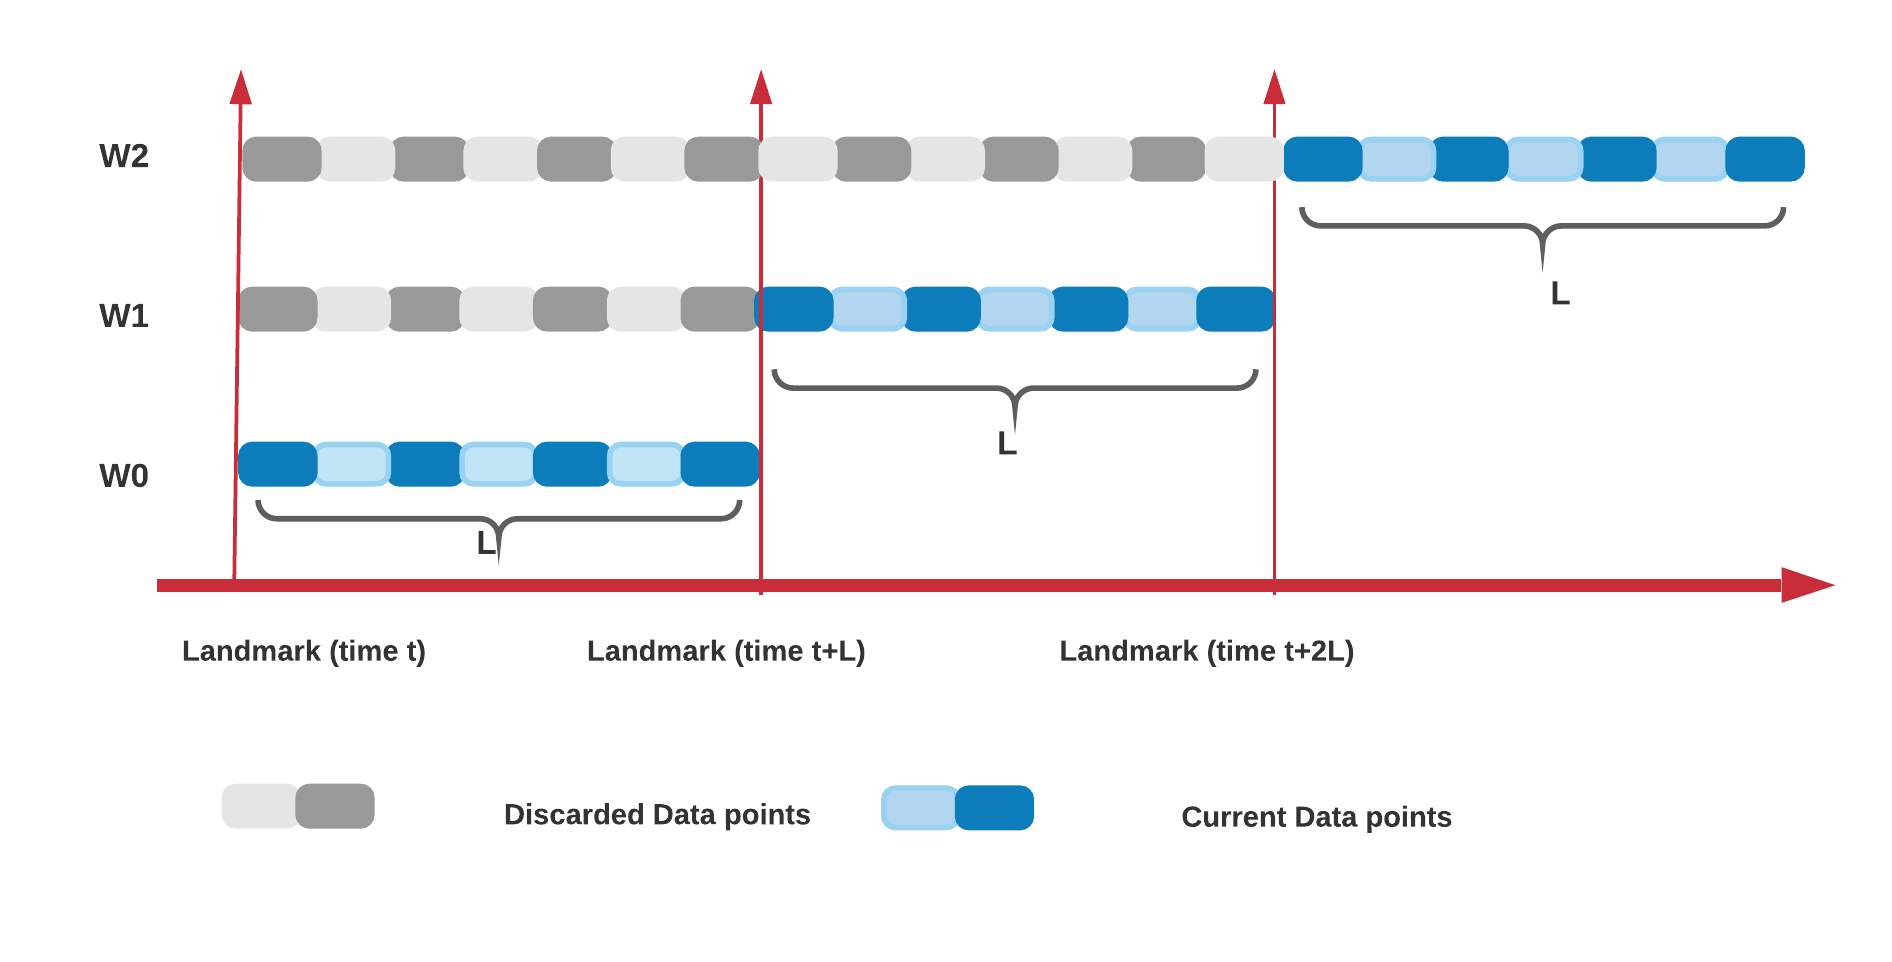
\includegraphics[width = 11 cm]{image/Chapters/Chapter4/LANDMARK-2.png}
    \caption{Landmark time window model }
    \label{land}
    \end{figure}
 
This online micro-cluster phase consists of three major steps: initialization, comparison, and activateAP and update $\epsilon_{W_j}$. %The tasks performed during these three steps are implemented in Algorithm 5.1 described in the next Chapter.

%If the next starting time is not available, we calculate the first time after the last time of the data in the window  [0][0].    
    % \[    \left [  s_{1} =\left ( E{1},N_{1},\sigma_{1},t{1} \right )  \right ], \left [ s_{2} = \left ( E_{2},N_{2},\sigma 2,t{1} \right ) \right ],\]
    % \[
    % ...,\left [ s_{i} = \left ( E_{i},N_{i},\sigma i,t{i} \right ) \right ] \] 


% Nei. Adding the last two phases, limited by free version.
  
    
    % Monica. Data Streaming with AP (STRAP): how the DSAP steps differ from STRAP steps???
    % Monica    
% 1. it does not have micro-macro clustering
% 2. using the slide time window (time duration) different from STRAP
    % Nei. Differences. 
    % 1. STRAP does not have micro-macro clustering phases. They claim that this makes the algorithm better than some of the others like Denstream since Strap always has an updated valid model while the others only maintain summaries(micro clusters). DSAP maintains the time history of data as micro clusters and updates the model (macro phase with time weighted micro clusters) periodically/user invoked like denstream.  
    % 2. DSAP employs Time windows on the data. The time dependence in STRAP comes only after the clustering/update stage where the older clusters are removed i.
    
    % 3. Model update. Once the reservoir is filled the AP restarts. But methodology to update the model are different. STRAP employs weighted clusters with some decay while DSAP adds an additional AP step so that only the cluster centroids are compared to update the prime centroids removing the need for a weights which would have added another potential variable. The decay of the centroids too will be different(currently not part of DSAP as you rightly pointed out in the last meting. I am leaning towards using the mechanism used by DBStream and SCluStream) 
    



% Monica. repository is equal to the TW, that is a problem....
% Nei: Old flowchart might have been confusing. The new version should fix this. The repository gets filled by points in any new time window that does not belong to any existing prime centroids. The repository consists of points over multiple time windows but within a reasonable time period that can be user defined and each point has a time dependent weight(still deciding) attached to it. This resolves the issue of older points corrupting the new model.

% Monica
% \begin{emph}
% {
% This section describes the StrAP algorithm, extending AP to Data Streaming,
% involving four main steps (Alg. 1):
% 1. The first bunch of data is used by ∗AP to compute the first exemplars and
% initialize the stream model. %Nei: The step names are similar hence it might have been confusing. The DSAP is inspired from Strap hence I kept the step names the same/similar for easy understanding. Initialization step. DSAP and Strap are the same. Ours is the first window from the sliding time window while Strap uses a bunch of points to find initial clusters.
% 2. As the stream flows in, each data item is compared to the exemplars; if too far from the nearest exemplar, it is put in the reservoir, otherwise the stream model is updated accordingly (section 3.1). % Nei: Update. This is similar between Strap and Dsap.
% 3. The restart criterion is triggered if the number of outliers exceeds the reservoir size, or upon a change point detection in the data distribution (section 3.2).% Nei: This step is called Restart criterion/Model rebuilding by Strap. We are calling this Activate AP step. The update criteria is different between Dsap and Strap. Change detection(data distribution change) not yet implemented in DSAP. 
% 4. If it is triggered, the stream model is rebuilt from the current exemplars and the reservoir, using ∗AP again (section 3.3). % Nei: Activate AP step. The stream model is rebuilt from the current exemplars(prime centroids) and reservoir centroids. This is different from Strap Model rebuilding phase.
% }
% \end{emph}

\begin{itemize}[leftmargin=*]
  

\item[]\textbf{Initialization}


The data stream is ingested in a windowed manner using the landmark time window model $W_0, W_1, ..W_j, ..,W_N $, where each window $W_j$ contains $\Omega$ data points and $L$ is defined as the time interval of window $W_j = [x_1,x_2...,x_i,..x_{\Omega}]$.

The clustering process is initiated by assigning the first sequence of data points from a data stream to the initial landmark time window $W_0$ as illustrated in Figure \ref{land}. The landmark time interval is a-priori determined based on user requirements, data rate, and expected latency of the expected data streams. For example, if high latency is expected in harvesting the data points, a long duration for the time intervals is advised. In contrast, in processing data from high rate streams, short time intervals will improve the clustering process. 

The AP algorithm is applied to the all data points belonging to the first time window $W_0$ for computing the initial micro-clusters and their respective centroids $C_m = C_{m_1}, C_{m_2},..C_{m_q}$. 

The micro-cluster centroids produced by the DSAP algorithm are represented as sequence of tuples:
    
    \[    \left [  s_{1} =\left ( C_{m_1},N_{1},t_{1} \right )  \right ], \left [ s_{2} = \left ( C_{m_2},N_{2}, t_{2} \right ) \right ],\]
    \[...,\left [ s_q = \left ( C_{m_q}, N_q, t_{q} \right ) \right ] \]  
    where
    \begin{itemize}
        \item[--] $C_{m_q}$ is the centroid of a micro-cluster $q$,
        \item[--] $N_q$ is the number of data points assigned to the cluster $q$, and
        \item[--] $t_{q}$ is the last timestamp assigned to the micro-cluster $q$.
    \end{itemize}

All data points within the initial landmark time window are considered as a potential exemplar until a robust set of centroids and their respective micro-clusters are found by computing the four AP matrices, i.e. similarity matrix, responsibility matrix, availability matrix and criterion matrix. The hyperparameters such as the preference parameter, the damping factor, the maximum number of iterations, and the convergence iteration are also set up during this phase. Their values will be constant throughout all the landmark time windows in the online micro-cluster phase.

A new hyperparameter $\epsilon_{W_j}$ is introduced in the DSAP algorithm for incrementally computing the clusters as time passes by, and as a result, allowing the analysis to take into account the changes of recurrently occurring clusters. For the initial time window $W_0$, an intra-cluster distance matrix is calculated between all data points and their respective centroids of each cluster using the Euclidean distance function. The mean of all these intra-cluster distances gives the initial value of the $\epsilon_{W_0}$ threshold that will be used in the next step.

The outputs of the initialization step are a set of micro-clusters centroids ($C_m$) and an initial $\epsilon_{W_0}$.


   
    
    % Monica. after you created a sequence of new TW with the same duration using a fixed time interval, and then for each TW you collect the data tuples, and compute the micro-cluster. 
    
    
    % The window is defined as a weight function of two variables, the time interval $t_i$ and the current time $t$.
    
    % \begin{equation*} W(t-t_{i}) = \begin{cases} 1, & \text {if }~t-t_{i} \le D \\ 0, & \text {if }~t-t_{i} > D \end{cases}\end{equation*}

    % As time passes, the window removes the tuples with the high time decay $D$. Then the recent data points are available to be clustered with the last time interval.
    
    
\item[]\textbf{Comparison}

As new data points arrive, the DSAP algorithm allocates them into their respective new time windows $W_j = [x_1,x_2...,x_i,..x_{\Omega}]$ using the same landmark time interval $L$ as defined in the previous step. For each new data point, a set of tasks are devised as follows:

\begin{itemize}
    \item[$\bullet$] Compute the Euclidean distances between each new data point $x_i$ and the current micro-cluster centroids $C_{m_q}$ using Equation \ref{eq1}.
    
    \begin{equation}
    d\left( C_{m_q},x \right)   = \sqrt { \sum_{1}^{n} \left( x_{i} - C_{m_{q_i}}\right)^2} \label{eq1}
   % d\left( C_{m_q},x_i \right)   = \sqrt {  \left( x_{i1} - C_m_{q1}\right)^2 + \left( x_{i2} - C_m_{q2}\right)^2 }, \label{eq1}
    \end{equation}

    where
    \begin{itemize}
        \item[--] $C_{m_q}$ is a current micro-cluster centroid,
        \item[--] $x$ is a new data point within the current landmark time window.
        \item[--] $x_{i}$ and $C_{m_{q_i}}$ are Euclidean vectors starting from the origin
        \item[--] $n$ space
    \end{itemize}
     
    
%The Euclidean distances between a centroid and the new data points starting from the origin are, $(C_m_{q1}, C_m_{q2})$ and $(x_{i1}, x_{i2})$ respectively.


    \item[$\bullet$] Compare the computed Euclidean distances against the current $\epsilon_{W_j}$. If one of the computed distance values is less than the current $\epsilon_{W_j}$ threshold (i.e. $min(d([C_{m}],x_i)) < \epsilon_{W_j}$), this new data point will be straightforward placed within a current existing cluster. The DSAP algorithm merges the new data point $x_i$ with the closest existing cluster by updating  the time $t_q$ and adding to the number of data points $N_q$ values in the cluster centroid tuple $C_{m_q}$. However, if all computed distance values are higher than the current $\epsilon_{W_j}$ threshold, the new points will be saved in the time-window repository temporarily until the landmark time window ends, and later be used in the next Activate AP and Update step.    
\end{itemize}

Figure \ref{thr} illustrates the previously described tasks by showing a sparse and a dense micro-cluster with their respective centroids $C_{m_i}$ and $C_{m_j}$. With a new data point $x_i$ arrival, the intra-cluster distances $T$ and $T'$ are computed in a time window $W_1$. In this case, the $T$ distance is less than the current $\epsilon_{W_1}$, and the new data point is merged to the existing cluster $C_{m_i}$ (Figure \ref{thr}a). In contrast, the computed distance $T'$ is greater than the current the current $\epsilon_{W_1}$ threshold, and this new data point will be saved in the time-window repository until the end of the streaming for the time window $W_1$ (Figure \ref{thr}b). These tasks take place every time a new landmark time window is created and new data points arrive.
%T' is chosen as the threshold for both clusters, it cannot assign all the data points which should belong to cluster with centroid $C_{mi}$. A threshold is computed dynamically according to the cluster evolution. In the data stream, the data is continuously changing, which necessitates an adaptive threshold $\epsilon_T$. In order to calculate this, first, the Euclidean distance between cluster centroids and all the data points in the same cluster are obtained. Then, the mean of all the distances gives the threshold value $\epsilon_T$. This adaptive threshold value uses for comparison in the next update step.
     
    \begin{figure}[!h]
    \centering
    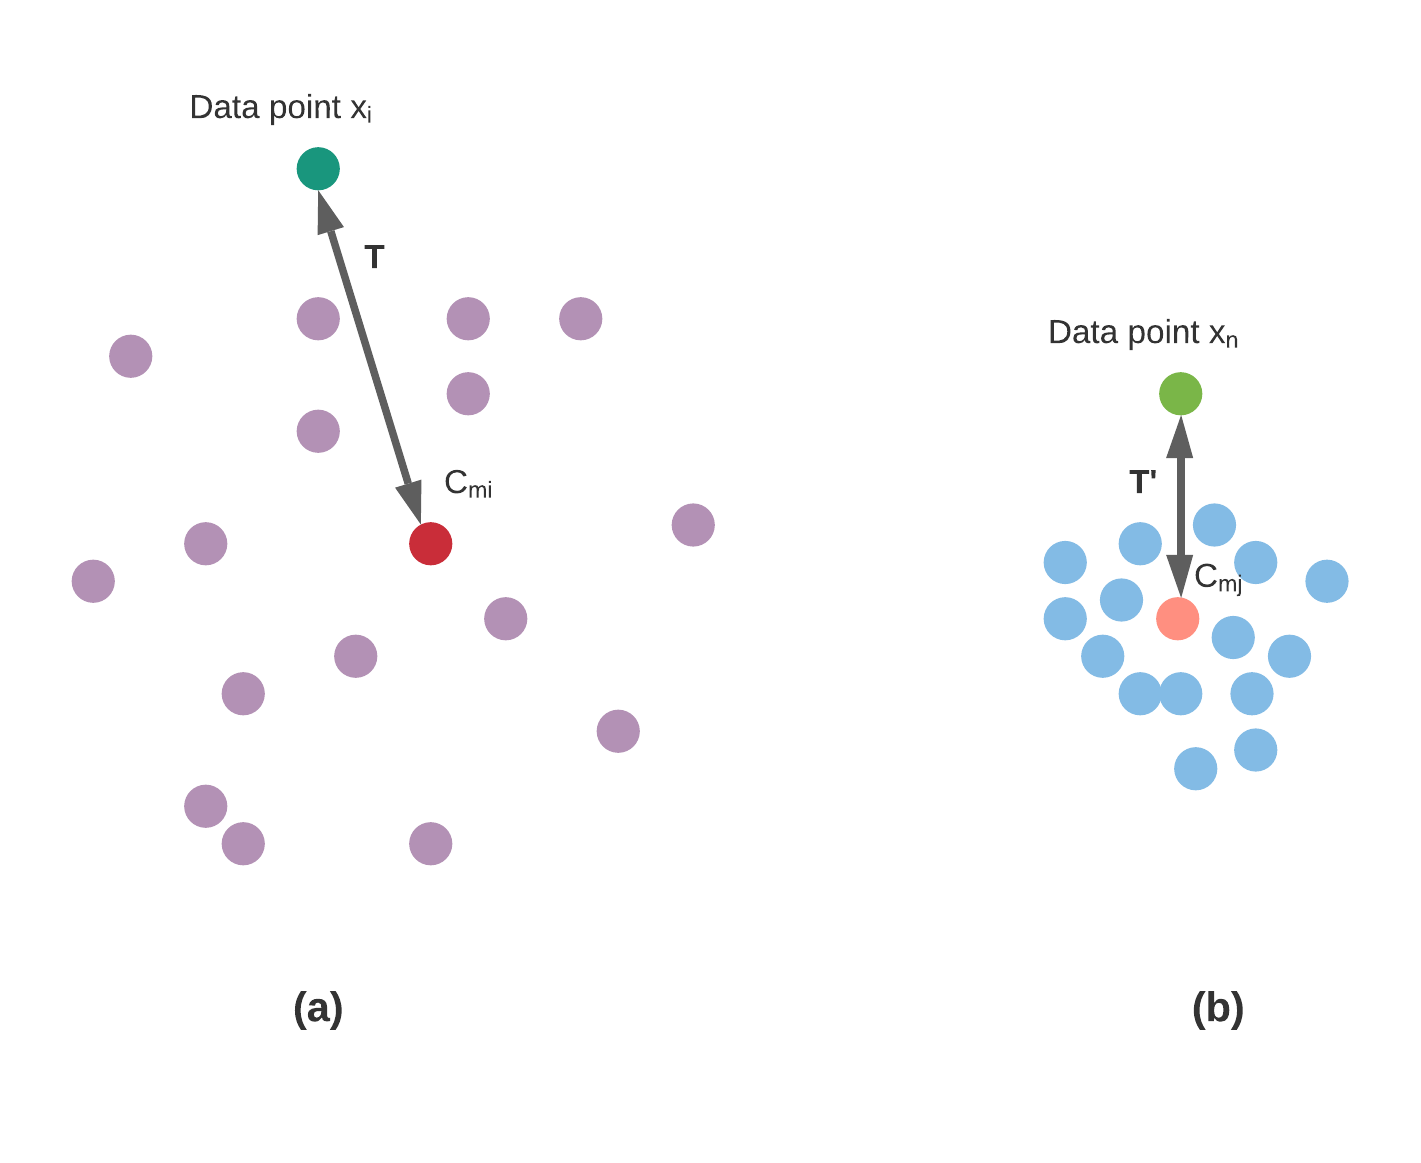
\includegraphics[width = 11 cm]{image/threshold.png}
    \caption{The impact of spread (a) and dense (b) cluster structures on comparing the closeness of new data points to existing micro-cluster centroids $C_m$ } 
    \label{thr}
    \end{figure}

The outputs of this step are the set of micro-clusters from the previous window, but now with new data points associated with some of the centroids, and an updated timestamp corresponding to the chosen centroids. Additionally, $n$ number of data points whose euclidean distance from the centroids was greater than $\epsilon_{W_j}$ are temporarily kept in the time-window repository.

%\todo[inline]{write down what the the outcomes are of this step}
    
    
    
\item[]\textbf{ActivateAP and Update  $\epsilon_{W_j}$}


    %The memory can fill up quickly if the data distribution changes. It is difficult to model a data stream with changing data distributions. This problem is referred to as concept-drift, that can lead to less accurate models as time passes. To handle concept-drift, the model needs to be consistently updated by moving the prime centroids of the clusters as the data evolves with time. Every once in a while when the number of data points in the repository exceeds a pre- defined value or at the end of the expiration time interval, the data points in the repository are clustered using AP. The expiration time ($T_{ex}$) is defined as time duration within which a data point stays relevant. It is set to a duration of $N_w$ times the window size ($T_{ex} = N_w*length(W_i)$) and is a user-defined parameter. After the AP is applied to the data points from the repository, new cluster centroids referred to as potential centroids ($[PC]$) are obtained. The potential centroids are compared with the prime centroids ($[C_{m0}]$). If the distance of any potential centroids from the prime centroids, $d(PC_i,Cm0_i)$ is less than the repository threshold $\gamma$ they will be grouped with the prime centroids for one final round of AP. This additional step of clustering centroids both prime and potential leads to the creation of new prime clusters as shown in Figure. \ref{frame}. Otherwise, if the distance is greater than the threshold, they will be added as a new prime centroid to the pool of prime centroids. After the AP is applied to the data points from the memory, new micro-clusters referred to as ($[PC]$) are obtained. This step of clustering leads to the creation of new micro-clusters. The outcome from this phase are a number of updated micro clusters ($C_{m0}$) that will be used to find macro clusters in the next phase.
    
   % new clusters are computed using the dta points which were stored in window 1
    
    
   % The data distribution changes over time. To have an accurate model as time passes, the model needs to be consistently updated as the data evolves with time.
    
    %All the data points in the current landmark window of length $L$ have been compared with the micro-clusters centroids, and if this distance is greater than the threshold, then the data point place in a temporary cache. 
    
    All the data points that have been temporarily accumulated during the execution of the previous step are used to compute new micro-clusters $C_m'$ using the AP algorithm once again. These new clusters will be added to the existing clusters $C_m$ that belong to their respective landmark time windows. As a result, the updated $C_m$ = $C_m'$ + $C_m$ is achieved. The new micro-clusters will have their respective timestamps associated with them.
    

    %Finally, these new clusters are added to the previous micro-clusters $Cm$, and the model is being updated ($Cm = Cm' + Cm$). 
    The next task is to compute the new $\epsilon_{W_j}$ by taking into account the centroids of the new micro-clusters found within a particular landmark window. This is accomplished by computing the mean of the intra-cluster distances using the new micro-clusters. The update $\epsilon_{W_j}$ is computed by applying the mean between the new and the current $\epsilon_{W_j}$. The updated $\epsilon_{W_j}$ is then used when the forthcoming data points from a new landmark time window arrive.
    
    
  
    
    %These points potentially represent new clusters. By applying the AP algorithm once again, new micro-clusters $Cm'$ are generated. Then, these new clusters $Cm'$ are added to the micro-clusters $Cm$ obtained before, and the model is updated ($Cm = Cm' + Cm$). The tasks performed during these steps are listed in Algorithm \ref{alg1} for better understanding.
    
  %\todo[inline]{how to get rid of old centroids... as soon as the centroids are not longer significant to compute the E , they are disregarded using the  factor. HOw do you do that??? } 

   In order to avoid the number of centroids to spread beyond control, old centroids that are no longer deemed relevant are removed. To do this, an expiration time parameter $e_x$ is introduced. This value is applied to forget centroids that haven't been selected in the recent windows as quantified by $e_x$. The $e_x$ number can be chosen to include all the time windows from the start or just the last few windows, depending on the user requirements. All the clusters whose associated timestamps are older than $e_x$ window lengths ($e_x \times L$) from the current time are considered obsolete and hence discarded. 
   %This value is obtained by subtracting the current time from the $ex$ number of time period. If any centroid in the previous time window seen in the current window, the timestamp associated to this centroid should be updated.
   
    % Increasing number of cluster usually lead to increasing time in processing the data, thus clustering process need to be broken down to prevent long process, this done by applying fading value to the process of clustering. 

% \begin{figure*}
% \centering
% \includegraphics[width = 15cm,height = 12cm]{image/tophase.png}
% \caption{The proposed DSAP flowchart }
% \label{frame}
% \end{figure*}



%After some time, the number of exemplars grows and maybe they become out of the control. To avoid this, we can remove the exemplar which has not been considered for a while. To implement this method, a specific time window $\triangle$ would be considered.
% \begin{equation}
%   \triangle_tj = t - t_j
%   \end{equation}

%After the new set of exemplars have been chosen, the list of outliers reset and new data points comes in to the model.


%%%%%%%%%%%%%%%%%%%%%%%%%%%%%%%%%%%%%%%%%%%%%%%%%%%%%%%%%%%%%%%%%%%%%%%%%%%%%%%%%%%%%%%%%%%%%%%%%
\end{itemize}


%need a table for notations and definitions! variables in the code
% which is illustrated in Figure \ref{frame} by the green box,
\subsection{Offline Macro-Cluster Phase}

The offline macro-cluster phase in DSAP, starts after $N$ time windows have passed. In this phase, all the micro-clusters $C_m$ generated during the online micro-cluster phase are re-clustered using the AP algorithm to generate $k$ number of macro-clusters $C_M = (C_{M_1}, C_{M_2}, ..., C_{M_k})$. This process is usually not considered time-critical and the number of macro-clusters are expected to be less than the number of micro-clusters. The hyperparameters related to the AP algorithm such as the the maximum number of iterations, and the convergence iteration are default values. The preference parameter is set to the median of the similarity matrix of all the micro-clusters obtained from the online phase, and the damping factor is fixed for all windows.


%\todo[inline]{Have you used the same hyperparameters??? Or they are changed??? e.g. number of interactions was the same for micro and macro clustering???} %Nasrin: No I don't change them. Just preference has been changed , which is the median of similarity matrix and I did not give it a number.

%The DSAP offline macro-clustering phase is composed of three steps. In the first step, the user requests for macro clusters from the online phase. Next, the list of micro clusters are retrieved from the online phase. The last step is to generate a set of macro clusters using the affinity-propagation clustering algorithm. AP gives macro clusters $[C_M]$ that summarizes all the micro clusters during the chosen interval. 




%The offline macro-clustering phase in DSAP,  which is illustrated in Figure \ref{frame} by green color, can be invoked by the user or pre-defined at regular intervals based on the data stream under consideration. In this phase, all the micro clusters $[C_{m0}]$ generated during the online phase are  re-clustered using another instance of the affinity propagation algorithm. The DSAP offline macro-clustering phase is composed of three steps. In the first step, the user requests for macro clusters from the online phase. Next, the list of micro clusters are retrieved from the online phase. The last step is to generate a set of macro clusters using the affinity-propagation clustering algorithm. AP gives macro clusters $[C_M]$ that summarizes all the micro clusters during the chosen interval. The pseudo-code presented in Algorithm \ref{alg1} succinctly summarizes the entire DSAP algorithm. 

%external: Rand index and Meila’s VI.
%One drawback of using internal criteria in cluster evaluation is the high scores on an internal measure do not truly result in data clustering. Additionally, this evaluation is biased towards algorithms that use the same cluster model. For example model used in k-Means clustering is naturally optimizes object distances, and a distance-based internal criterion will likely misjudge the resulting clustering.




\section{Intrinsic Clustering Validation Phase} \label{intrinval}

Intrinsic clustering validation uses the internal information of the clustering process to evaluate the goodness of a clustering structure when the ground truth labels are unknown. The well-known metrics silhouette index (S),  Caliński-Harabasz index (CH), and Davies-Bouldin index (DBI) were selected to validate the goodness of macro clusters found by the DSAP algorithm. Table \ref{comp} provides an overview of these metrics. They are further described in detail in the following sections.

%\todo[inline]{have you computed the metrics for micro and macro clusters??? or just macro clusters??} %Nasrin: Just Macro clusters

% \begin{table}[htbp]\scriptsize
% % \centering
% \caption{Intrinsic clustering metrics used for validation of clustering results.}
% \label{comp}   
% \begin{tabularx}{\linewidth}{|p{2cm}|p{5cm}|p{3cm}|p{3.4cm}|}
% \hline
%  \multicolumn{1}{|c|}{\textit{\textbf{Metric}}} &
%  \multicolumn{1}{|c|}{\textit{\textbf{Description}}} &
%  \multicolumn{1}{|c|}{\textit{\textbf{Advantages}}}   &   
% \multicolumn{1}{|c|}{\textit{\textbf{Disadvantages}}} 
% \tabularnewline \hline
% \vfill 
%  \raggedright Silhouette Index &  
% \vfill
%  It measures how similar a data point is to its own cluster compared to other clusters.
%  &
 
%  \begin{enumerate}[*,nosep,leftmargin=0.2cm]
%  \item Value bounded between [-1,1]  
%  \item High scores when clusters are well separated
% \end{enumerate}
% \tabitem
% &       
% \begin{itemize}[*,nosep,leftmargin=0.2cm]
%     \setlength\itemsep{0em}
%      \item High computational complexity
%      \item Higher value for convex clusters unlike density based clusters
% \end{itemize} 
% \tabularnewline \hline
% \vfill 
%  Caliński-Harabasz Index     &     
% \vfill
% It is the ratio between the intra-cluster dispersion and the inter-cluster dispersion.
% & 
% \begin{itemize}[*,nosep,leftmargin=0.2cm]
%     \item Fast to compute
%     \item Easy to interpret %as it gives higher value when clusters are dense
% \end{itemize}
%  &       

% \begin{itemize}[*,nosep,leftmargin=0.2cm]
%     \item Higher value for convex clusters% compared with density based clusters
% \end{itemize}
% \tabularnewline \hline
% \vfill 
% Davies-Bouldin Index        &       
% \vfill
% It is the average similarity measure of each cluster with its most similar cluster.%, where similarity is the ratio of within-cluster distances to between-cluster distances
% & 
% \begin{itemize}[*,nosep,leftmargin=0.2cm]
%     \item Simple to implement
%     \item Value is able to compute when features inheritent to the dataset
%     %\item Quantity computation ?????
% \end{itemize}
%          &      
         
% \begin{itemize}[*,nosep,leftmargin=0.2cm]
%     \item Higher values for convex clusters
%     \item Limited to Euclidean distance only
% \end{itemize}

% \tabularnewline\hline

% \end{tabularx}
% \end{table}
%%%%%%%%%%%%%%%%%%%%%%%%%%%%%%%%%%%%
\begin{table}[htbp]
\small
\caption{Intrinsic clustering metrics used for validation of clustering results.}
\label{comp}
\begin{tabular}{llll}
\hline
\multicolumn{1}{c}{\textbf{Metrics}}                                  & \multicolumn{1}{c}{\textbf{Description}}                                                                                                 & \multicolumn{1}{c}{\textbf{Advantages}}                                                                                                          & \multicolumn{1}{c}{\textbf{Disadvantages}}                                                                                                                  \\ \hline\midrule
\begin{tabular}[c]{@{}l@{}}Silhouette\\  Index\end{tabular}           & \begin{tabular}[c]{@{}l@{}}It measures how similar\\ a data point is to its own\\ cluster compared to \\ other clusters.\end{tabular} & \begin{tabular}[c]{@{}l@{}}* Value bounded \\  between {[}-1,1{]}\\ * High scores when \\ clusters are well\\  separated\end{tabular}             & \begin{tabular}[c]{@{}l@{}}* High computational\\    complexity\\ * Higher value for \\    convex clusters  unlike\\    density-based clusters\end{tabular} \\ \hline
\begin{tabular}[c]{@{}l@{}}Caliński-\\ Harabasz \\ Index\end{tabular} & \begin{tabular}[c]{@{}l@{}}It is the ratio between\\ the intra-cluster \\ dispersion and the\\ inter-cluster dispersion.\end{tabular}    & \begin{tabular}[c]{@{}l@{}}* Fast to compute\\ * Easy to interpret\end{tabular}                                                                  & \begin{tabular}[c]{@{}l@{}}* Higher value for\\    convex clusters\end{tabular}                                                                             \\ \hline
\begin{tabular}[c]{@{}l@{}}Davies-\\ Bouldin\\  Index\end{tabular}    & \begin{tabular}[c]{@{}l@{}}It is the average\\  similarity  measure\\ of each cluster with \\ its most similar cluster.\end{tabular}     & \begin{tabular}[c]{@{}l@{}}*Simple to implement\\ *Value is able to com-\\    pute when features\\    inherent to the \\    dataset\end{tabular} & \begin{tabular}[c]{@{}l@{}}* Higher values for \\    convex clusters\\ * Limited to Euclidean\\    distance only\end{tabular}                               \\ \hline\midrule
\end{tabular}
\end{table}








\subsection{Silhouette Index}

 The silhouette index was introduced by \cite{rousseeuw1987silhouettes} on the premise of the  silhouette  width  of  a  data  point to measure how similar a data point is to its own cluster compared to other clusters. The silhouette index $S_i$ for a data point $i\in x$ in cluster $C_k\in C$ is calculated using Equation \ref{sil}.
 
 %\todo[inline]{missing reference rousseeuw1987silhouette}
 
 \begin{align}
    a_i = \frac{1}{C_k} \sum_{j \in C_k,i\neq j } d(i,j) \\
    b_i = \min_{C_m \in C, C_m\neq C_k} \frac{1}{\abs{C_m}} \sum_{j \in C_m,i\neq j} d(i,j) \\
    s_i =  \frac{b_i - a_i}{\max(a_i,b_i)}  \label{sil}
\end{align}

The first parameter $a$ is the average distance between the sample and all the others in the same class, and the second parameter $b$ is the mean distance between the sample and all the other points in the next closest cluster. Negative $S_i$ scores for a point $i$ means that the data point is in the incorrect cluster. Positive scores show a robust and dense clustering. Moreover, values around zero indicate overlapping clusters. If the $S_i$ has a higher value, it means a greater ratio between $b_i$ as compared with $a_i$, causing the data point $i$ to be more similar to the other data points in the same cluster.  

The primary advantage of the silhouette index is its straightforward interpretation. The score is bounded between -1 for incorrect clustering and +1 for highly dense clustering. Scores around zero indicate overlapping clusters. The score is higher when clusters are dense and well separated, which relates to a standard concept of a cluster. However, it has a high computational complexity of $O(n^2)$. Additionally, it is well known that the coefficient values tend to be higher for convex clusters as compared to other uniquely shaped density based clusters.


%\begin{figure}
    %\centering
   % 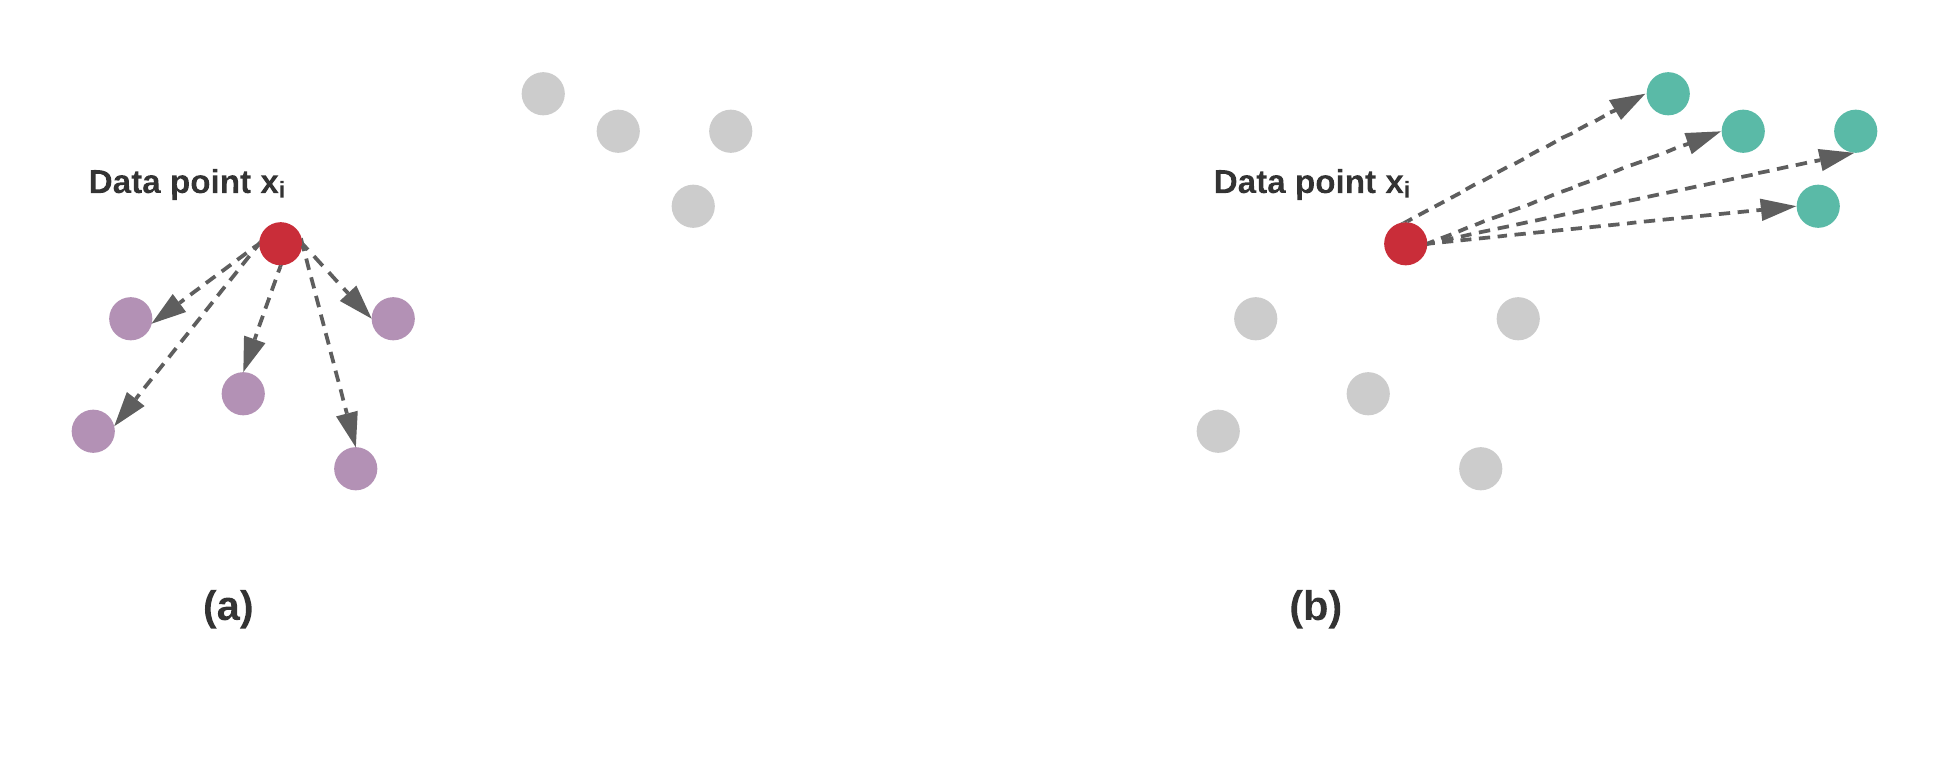
\includegraphics[width = 11 cm]{image/silo.png}
   % \caption{Silhouette Coefficient for a data point $x_i$, calculates for all data points in its own cluster(a), and for all other data points in other clusters (b).}
   % \label{silo}
%\end{figure}
    

\subsection{Caliński-Harabasz Index}
It is also known as the variance ratio criterion, which is used to score dense and well-separated clusters. A recent comparative study of available clustering indices demonstrated this index as one of the best cluster validity indices \cite{arbelaitz2013extensive}. 

%\todo[inline]{not sure if you have cited this paper}%Fixed it

Well defined clusters yield high values of this index. Therefore, the maximum value of the index is used to select the best partition. For \begin{math} n \end{math} data points, \begin{math} k \end{math} clusters  where \begin{math} B \end{math} and \begin{math} W \end{math} are the between within cluster scatter matrices, the index is computed as \cite{calinski1974dendrite}:

%\todo[inline]{not sure why the reference calinski1974dendrite is not being compiled}

\begin{equation}
  CH =  \frac{traceB / (k - 1)} {traceW/ (n -k)}
\end{equation}   


%For a  data point $i$ of size $I$ which has been clustered into $k$ clusters, the Calinski-Harabasz score $s$ is defined as the ratio of the mean dispersion between clusters and the within cluster dispersion:

%\begin{equation}
    %s = \frac{\mathrm{tr}(B_k)}{\mathrm{tr}(W_k)} \times \frac{n_i - k}{k - 1}
%\end{equation}
where
\begin{equation}
    B_k = \sum_{q=1}^k n_q (c_q - c_i) (c_q - c_i)^T
\end{equation}

\begin{equation}
    W_k = \sum_{q=1}^k \sum_{x \in C_q} (x - c_q) (x - c_q)^T
\end{equation}

with $C_q$ the set of points in cluster $q$, $c_q$ the center of cluster $q$, $c_D$ the center of $D$, and $n_q$ the number of points in cluster $q$.

%The $tr(B_k)$ is a dispersion matrix effect between groups of data and $tr(W_k)$ is the effect of the within-cluster dispersion matrix defined by $B-k$


The CH is computationally efficient to calculate, but just like the silhouette index, the CH index is biased towards convex clusters assigning them higher values than the density based clusters such as those obtained through DBSCAN.

\subsection{Davies-Bouldin Index}

Davies-Bouldin Index (DBI) was introduced in 1979 by \cite{4766909}, and it computes the average similarity between each cluster $C_i$ for $i = 1,2,...,k$ and its most similar one $C_j$.  For this index, similarity is defined as a measure $R_{ij}$ that optimizes:

\begin{itemize}
    \item $s_i$: the average distance between each data point in the cluster and the centroid of that cluster.
    \item $d_{ij}$: the distance between cluster centroids $i$ and $j$.
\end{itemize}

A simple choice to construct $R_{ij}$ is that of non-negative and symmetric as follows:

\begin{equation}
    R_{ij} = \frac{s_i + s_j}{d_{ij}}
\end{equation}

Then the Davies-Bouldin index is defined as:

\begin{equation}
    DB = \frac{1}{k} \sum_{i=1}^k \max_{i \neq j} R_{ij}
\end{equation}

 With this index, a minimum value denotes the best partitioning of the data. The average similarity calculation is much simpler than the computations required for calculating the silhouette index. Like the previous two metrics, DBI too suffers from a preference towards convex clusters as compared to density based clusters owing to the usage of centroid distance that limits the distance metric to Euclidean space.





% \subsection{Comparison of Intrinsic Clustering Metrics}
% The three metrics discussed above have some advantages and drawbacks which they are listed below.
% \begin{itemize}
%     \item The advantage of using the Silhouette Coefficient is this score has a range between -1 and 1. The high score shows that the data point is well matched to its own cluster and clusters are dense, and the low value shows a poor match to the neighboring clusters. On the other hand, the Silhouette Coefficient is a data-related metric, and it means it is higher for convex clusters than other types of clusters such as density based clusters like DBSCAN. Also, the time complexity for this score is $O(n^2)$ which is high.
    
%     \item The advantage of applying the Calinski-Harabasz Index is it is fast to compute the number, and it shows the density of the clusters with a higher value, which is related to the concept of a cluster. However, the drawback is this score is mostly higher when the clusters are convex.
    
    
%     \item The advantage of having Davies-Bouldin Index is that computing this metric is simpler than computing the Silhouette Coefficient. Also, this value is able to compute when features inheritent to the dataset. 
%     The drawback of the index is as the other metrics mentioned before, is being higher for convex clusters such as density based clusters like DBSCAN, and 
%     (change)the usage of centroid distance limits the distance metric to Euclidean space.
% \end{itemize}



% Please include the text below:
% Comparison between these metrics:

% Silhouette Coefficient
% Advantages
%     The score is bounded between -1 for incorrect clustering and +1 for highly dense clustering. Scores around zero indicate overlapping clusters.

%     The score is higher when clusters are dense and well separated, which relates to a standard concept of a cluster.

% Drawbacks

%     The Silhouette Coefficient is generally higher for convex clusters than other concepts of clusters, such as density based clusters like those obtained through DBSCAN.

%     High computational complexity: O(n²)
    
    
% Calinski-Harabasz Index
% Advantages
%     The score is higher when clusters are dense and well separated, which relates to a standard concept of a cluster.

%     The score is fast to compute.

% Drawbacks

%     The Calinski-Harabasz index is generally higher for convex clusters than other concepts of clusters, such as density based clusters like those obtained through DBSCAN.

% Davies-Bouldin Index
% Advantages
%     The computation of Davies-Bouldin is simpler than that of Silhouette scores.

%     The index is computed only quantities and features inherent to the dataset.

% Drawbacks
%     The usage of centroid distance limits the distance metric to Euclidean space.

%     The Davies-Boulding index is generally higher for convex clusters than other concepts of clusters, such as density based clusters like those obtained from DBSCAN.


%\item\textbf{Clustering-based Outlier Detection:}
%The purpose of outlier detection is to separate a core of general observations from the polluting ones or outliers. They can be noise or an interesting data points and in both cases outlier detection is important. Also the number of outliers have a relationship with the model efficiency. These outliers can effect the quality of the model and the centroids of each clusters. Either these data points do not belong to any other clusters or to the clusters which are far from other clusters. To find how the DSAP is efficient in detecting outliers, we inject specific number of data points to our algorithm to see how it can affect our result. 

% To find out which algorithm is support robust in terms of  outliers, Support Vector Data Description (SVDD) algorithm is employed by generating hyper sphere for the data.  
%Based on the Equation \ref{out}, if $O_i$ is the $i^{th}$ cluster, $|O_i|$ be cardinality of $O_i$ and $j$ is the cluster count, then $O_m$ is the outlier if: 
% \begin{equation}
%     \abs{O_m} << \frac{1}{j} \sum_{i=1}^{j} \abs{O_i}\label{out}
% \end{equation}

\section{Clustering Performance Evaluation Phase}

Data stream clustering brings about a few unique challenges as compared to traditional data clustering. The data streams are a continuous flow of data points that arrive at rapid rate. Random access to these data points is not possible and the volatility of the data streams sometimes limits to having a single look at the data points upon their arrival. 

%As a result there is a need for fast processing of each data point that arrives from the stream and maintain summaries of the data instead of the raw data to save memory. 

To evaluate the efficiency of the DSAP, two metrics are proposed: computational time and the memory consumed to run the DSAP algorithm. These metrics used in this phase are described in the next sections.

\subsection{Time Complexity}

The efficiency of any algorithm can be estimated using the time complexity, which can be defined as the time taken to run the number of elementary operations performed by the algorithm given an input array of length N. In other words, it is the amount of time taken by an algorithm to run, as a function of the length of the input.  

The most frequently performed action within the algorithm whose execution time does not change with the size of the input array is called the elementary operation. The most common metric used for estimating time complexity is the Big O notation. The big O notation is typically used to illustrate the worst-case growth of an algorithm (or how the run time/space requirements of an algorithm increase with input size), which excludes coefficients and lower order terms.

In real-world applications, in addition to the time complexity, several other factors can affect the execution speed. Many concurrent tasks like receiving network traffic, checking the hard disk, and writing log files, are performed by a typical computer while it performs the clustering tasks. The data-dependent rate of convergence of the algorithms also affects the total execution time. Therefore, it is recommended to run a task multiple times to get average values after discarding the initial few results as they could be affected by the time-window repositoryd results. %Plot the spread over multiple runs to choose a cutoff.
%Rough estimates of the start and end times of the algorithms can be noted by native functions available under each programming language.


\subsection{Space Complexity} 
Similar to the time complexity, the memory consumption quantifies the amount of memory taken by an algorithm to run as a function of the length of the input. That means how much memory, in the worst case, is needed at any point by the algorithm. The same big-O notation is used to describe the space complexity as well. This parameter represents the algorithm’s scalability and performance. In simple terms, it gives the worst-case scenario of an algorithm’s growth rate.

To calculate space complexity, we need to know the value of memory used by different types of datatype variables, which generally vary for different operating systems. Hence it is not straightforward to provide generic formulations for the spatial complexity of any algorithm.

To compare different algorithms, we have to make sure that they have been suitably implemented since poor memory management can lead to a superior algorithm under-performing as compared with the superior implementation of a less efficient algorithm. Analogous to the time metric, it is necessary to test the algorithms on data sets of multiple sizes for an accurate assessment of the memory usage. 


% \section{Comparison  Between  DSAP  and  Streaming  K-means Phase}

% move the paragraphs here to other sections

% - difficult to find available source code for previusouly proposed stream AP, etc...


% The general approach of the various stream clustering algorithms that allow for the investigation of the cluster structure at different time intervals are fairly similar. They typically have two stages, online where the algorithm maintain a summary of the data as micro-clusters and next in the offline phase the summary micro-clusters are clustered to provide real insights to the data. The efficiency of these algorithms are greatly affected by the choice of the clustering algorithm used. We have introduced the DSAP algorithm for data stream clustering which is implemented based on the AP algorithm. This model is compared with the established streaming K-means algorithm introduced earlier in Chapter 2. It is known that the AP algorithm usually generates results that show that the k-means algorithm is faster than AP. However, streaming AP based algorithms has been shown to provide similar quality clusters as k-means based ones but, the results tend to be more robust.

% K-means algorithm is scalable for large datasets with different shapes and sizes and is easy to implement. The K-means algorithm is known to easily adopt to new centroids and is one of the fastest algorithms out there owing to a linear time complexity. Also, K-means guarantees convergence by trying to minimize the total sum of the square error as an objective function over the number of iterations. On the other hand, the K-means algorithm has some known drawbacks. Finding the $k$ optimum number of clusters is not a precise task that can be accurately automated. The algorithm results are a function of the initial clusters chosen and necessitate multiple runs of the algorithm with the different values to pick the most suitable clusters. During data stream clustering this process can be time consuming and make the model less accurate. The algorithm is known to have difficulties in finding the right clusters for data with varying size and density. In addition, K-means clusters centroids are affected by outliers since the mean as a statistic is sensitive to outliers. %it means outliers can drag the centroids or they may have their own centroids. 
% Lastly, even though K-means can be easily scaled to large datasets but it has difficulties to cluster high-dimension data. 


% In comparison with the K-means algorithm that needs to determine the optimal number of clusters prior by applying some methods like elbow method, the AP algorithm calculates the number of clusters internally. However, AP needs additional parameters like the damping factor and preference to be set since the model convergence is dependent on the damping parameter while the preference controls the probability of finding centroids. Due to the additional complexities in the calculation of AP it becomes prohibitively expensive to scale AP as compared to the K-means which scales linearly with the size of the dataset. The semi-supervised selection of the number of clusters in K-means limits the potential of producing large number of clusters that can sometimes be generated by the AP if it's parameters are not chosen carefully. Both these partitioning based algorithms can be evaluated based on metrics that quantify the density and spread of the clusters. 

% Affinity propagation has been shown to perform well in pattern recognition applications in the fields of computer vision and computational biology. The main advantage of AP is the robustness of its optimization. While K-means follows a greedy optimization method to find the optimum of the optimization problem, AP tackles a continues optimization problem, in which all data points are potential candidate at the beginning and clusters are gradually identified. AP does not suffer from the initialization can guarantee global optimization consistently.

\section{Summary}

Figure \ref{frame} summarizes the entire research methodology discussed in this chapter. The four phases of the DSAP approach are depicted with their main steps and respective tasks. 



%were discussed. Figure based on four phases is introduced along with the various quality and performance evaluation techniques. This algorithm consists of two phases, online micro-cluster and offline macro-cluster. These two phases are depicted with the grey and green boxes in the flow chart shown in Figure \ref{frame} that summarizes the entire research methodology discussed in this chapter. The online phase finds the updated micro-clusters from the stream by applying landmark window. The offline phase generates macro-clusters, a summary of all data points from the stream by re-clustering the micro-clusters. 

\begin{figure}[h]
\centering
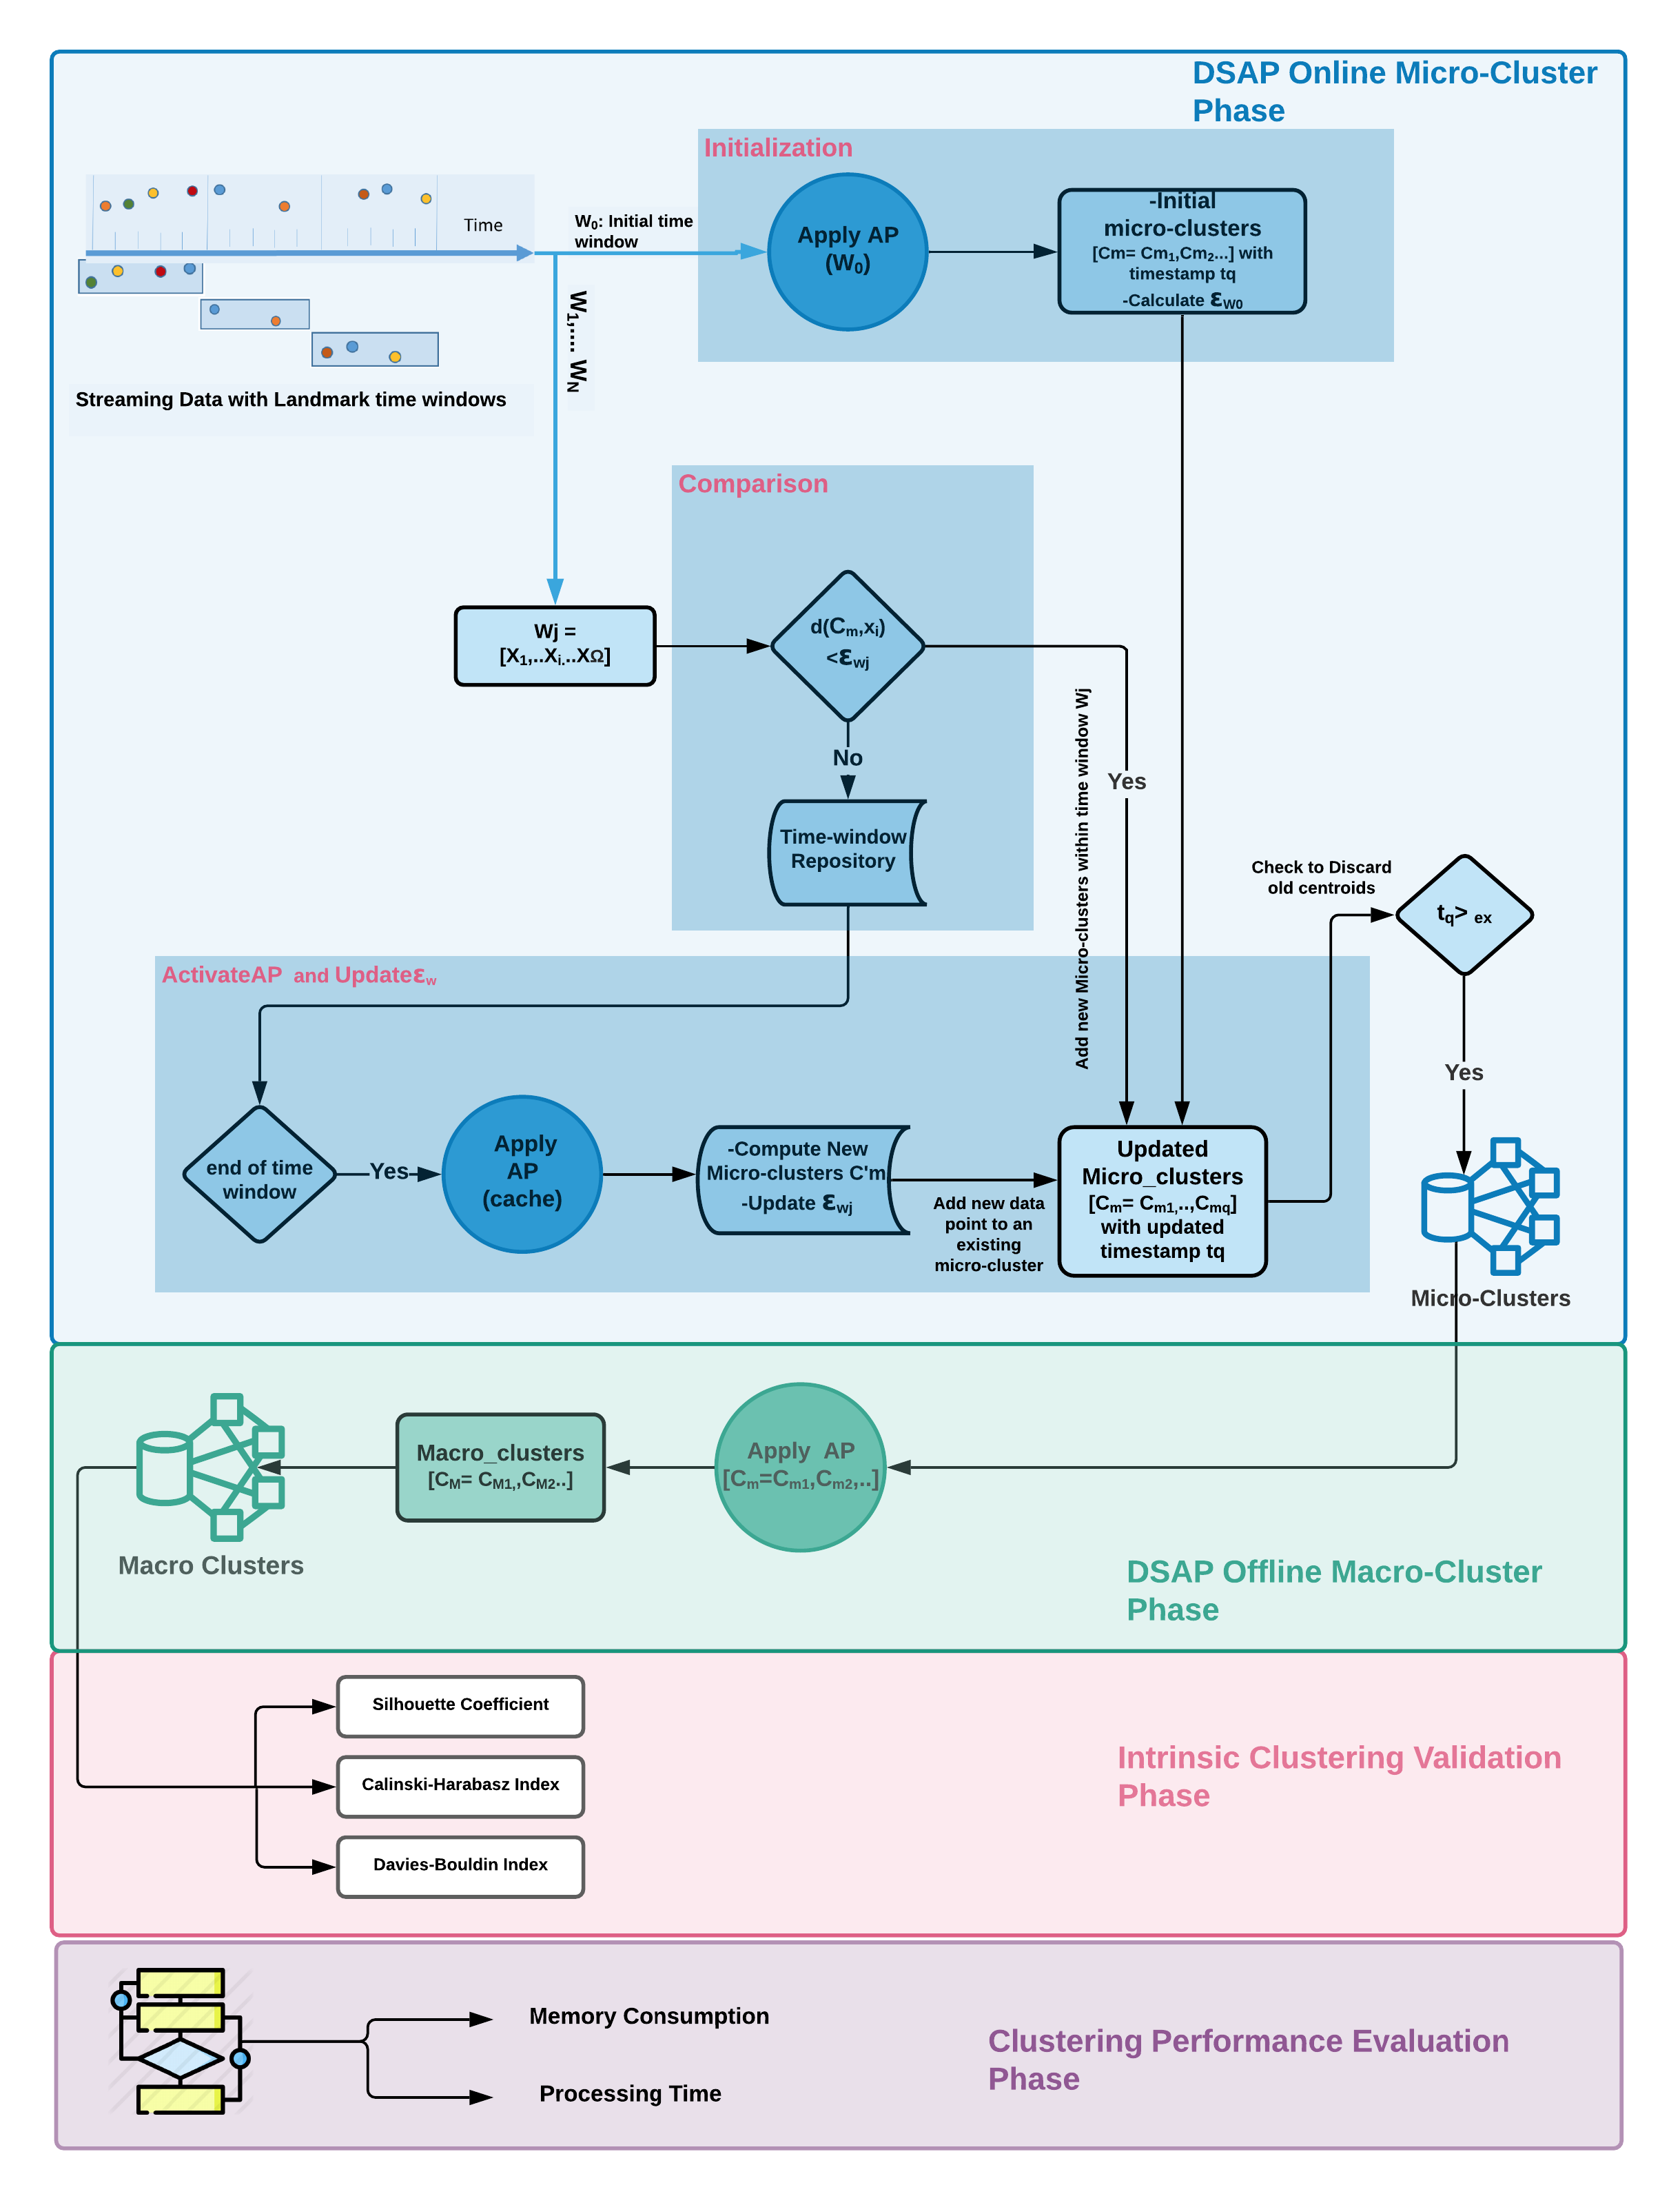
\includegraphics[width =1.05\textwidth]{image/Chapters/Chapter4/dsapflowchart1.png} 
\caption{Flowchart of the proposed DSAP approach}
\label{frame}
\end{figure}

The online micro-cluster and offline macro-cluster phases are are depicted within the grey box in blue and green colors respectively in the flow chart shown in Figure \ref{frame}. The online phase initializes the computation of micro-clusters and computes the updated micro-clusters from the new data points harvested using the landmark time window. The offline phase generates macro-clusters, a summary of all data points from the stream by re-clustering the micro-clusters. 

The silhouette index, Caliński-Harabasz index, and Davies-Bould in index are proposed to assess the goodness of  the clustering structures of the discovered micro and macro clusters since the ground truth labels were unknown. This phase is illustrated in Figure \ref{frame} with bright red color. The efficacy of any stream clustering algorithm is tied to its memory consumption and speed of execution. In order to evaluate this, in the Clustering Performance Evaluation phase shown in Figure \ref{frame} with purple color, the time and space complexity of the DSAP algorithm are estimated. 



















% Monica. EXPLAIN WHY THIS COMPARISON IS IMPORTANT
% 1. AP has usually produced results that have shown the k-means was faster than AP
% 2. However DSAP has shown to provide similar performance as k-means

% ---------------------- source https://developers.google.com/machine-learning/clustering/algorithm/advantages-disadvantages -------------------------------------
% -----------------------
% Advantages of k-means : Scales to large data sets. Guarantees convergence. Can warm-start the positions of centroids. Easily adapts to new examples. Generalizes to clusters of different shapes and sizes, such as elliptical clusters.

% Disadvantages of k-means
% Choosing  manually.

% Use the “Loss vs. Clusters” plot to find the optimal (k), as discussed in Interpret Results.

% Being dependent on initial values.

% For a low , you can mitigate this dependence by running k-means several times with different initial values and picking the best result. As  increases, you need advanced versions of k-means to pick better values of the initial centroids (called k-means seeding). For a full discussion of k- means seeding see, A Comparative Study of Efficient Initialization Methods for the K-Means Clustering Algorithm by M. Emre Celebi, Hassan A. Kingravi, Patricio A. Vela.

% Clustering data of varying sizes and density.

% k-means has trouble clustering data where clusters are of varying sizes and density. To cluster such data, you need to generalize k-means as described in the Advantages section.

% Clustering outliers.

% Centroids can be dragged by outliers, or outliers might get their own cluster instead of being ignored. Consider removing or clipping outliers before clustering.



% -----------------------
% DIFFERENCES BETWEEN K-MEANS AND AP

% Differences between K-means and affinity propagation:

% Parameters on initialization:
% KM: number of clusters.
% AP: damping damps the responsibility and availability messages, sample preference controls the number of exemplars.
% Scalability:
% KM: scalable with the number of samples.
% AP: not scalable with the number of samples.
% Usecase:
% KM: General-purpose, even cluster size, flat geometry, not too many clusters.
% AP: Many clusters, uneven cluster size, non-flat geometry.
% Metric used:
% Distances between points.
% Graph distance.
% Application:

% Affinity propagation was shown to perform well on the following tasks:computer vision.
% biology tasks.
% -----------------------------------------------

% ADVANTAGES OF AP: Affinity Propagation is much more
% tolerant to errors, it can remove the oscillation when it occurs
% where the occupance of oscillation will bring the algorithm to fail
% to converge. Adaptive Affinity propagation is more stable than
% the other since it can deal with error which the other can not.
% And Fuzzy Statistic Affinity Propagation can produce smaller
% number of cluster compared to the other since it produces its
% own preferences using fuzzy iterative methods.
% --------------------------------------------


% \end{document}


% the drawback of applying K-means clustering algorithm is that is need to calculate the number of clustre prior 

 % \begin{equation}
    % d^i_{min}   = min [{d(E^{i-1}_{m}, W^i), d(E^{i-1}_{m'}, W^i)}]
    % \end{equation}
    %To control the number of centroids to not exceed beyond the control, the old centroids have not visited for a long time, should be remove. To do this, the centroids will be deleted over the time. 
    % wite inja  tedad marakez ziad beshe
    
    %\item\textbf{re-establishing:}
    %add the decay value: This repository has the latest window and is identified by the decay factor.